\makeatletter
\def\@ecole{école}
\newcommand{\ecole}[1]{
  \def\@ecole{#1}
}

\def\@specialite{Spécialité}
\newcommand{\specialite}[1]{
  \def\@specialite{#1}
}

\def\@ED{\'{E}cole Doctorale}
\newcommand{\ED}[1]{
  \def\@ED{#1}
}

\def\@doctorat{Doctorat}
\newcommand{\doctorat}[1]{
  \def\@doctorat{#1}
}

\def\@adresse{Adresse}
\newcommand{\adresse}[1]{
  \def\@adresse{#1}
}

\def\@directeur{directeur}
\newcommand{\directeur}[1]{
  \def\@directeur{#1}
}

\def\@encadrant{encadrant}
\newcommand{\encadrant}[1]{
  \def\@encadrant{#1}
}
\def\@jurya{}{}{}
\newcommand{\jurya}[3]{
  \def\@jurya{#1,	& #2	& #3\\}
}
\def\@juryb{}{}{}
\newcommand{\juryb}[3]{
  \def\@juryb{#1,	& #2	& #3\\}
}
\def\@juryc{}{}{}
\newcommand{\juryc}[3]{
  \def\@juryc{#1,	& #2	& #3\\}
}
\def\@juryd{}{}{}
\newcommand{\juryd}[3]{
  \def\@juryd{#1,	& #2	& #3\\}
}
\def\@jurye{}{}{}
\newcommand{\jurye}[3]{
  \def\@jurye{#1,	& #2	& #3\\}
}
\def\@juryf{}{}{}
\newcommand{\juryf}[3]{
  \def\@juryf{#1,	& #2	& #3\\}
}
\def\@juryg{}{}{}
\newcommand{\juryg}[3]{
  \def\@juryg{#1,	& #2	& #3\\}
}
\def\@juryh{}{}{}
\newcommand{\juryh}[3]{
  \def\@juryh{#1,	& #2	& #3\\}
}
\def\@juryi{}{}{}
\newcommand{\juryi}[3]{
  \def\@juryi{#1,	& #2	& #3\\}
}
\makeatother

\newcommand\BackgroundPic{%
	\put(0,0){%
		\parbox[b][\paperheight]{\paperwidth}{%
			\hspace{5em}
			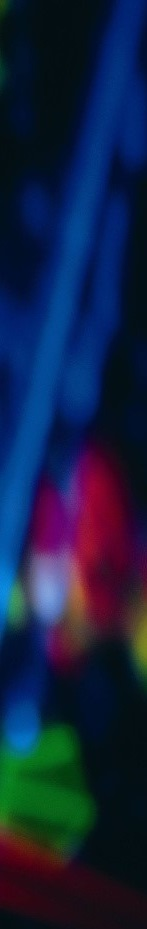
\includegraphics[height = 0.45\paperheight]{Illustrations/Bordure}%
			\vfill
		}
	}
}

\definecolor{ensamcolor}{rgb}{0.56,0.14,0.38}

\newcommand\EtiquetteThese{%
%Ici c'est le positionnement de l'encadré en bas à droite
	\put(-20,65){% c'est le point bas droite
		\parbox[t][\paperheight]{\paperwidth}{%
			\hfill
			\colorbox{ensamcolor}{		
				\begin{minipage}[b]{3em}
				\vspace{0.3cm}        %ça c'est bon
					\centering\Huge\textcolor{white}{T\\H\\\`{E}\\S\\E\\}
					\vspace{0.3cm} %ça c'est bon
				\end{minipage}
			}
		}
	}
}

\makeatletter
\newcommand{\pagedegarde}{
 \newgeometry{top=0.8cm, bottom=1cm, left=2cm, right=1cm}
 \AddToShipoutPicture*{\BackgroundPic}
 \AddToShipoutPicture*{\EtiquetteThese}
   \begin{titlepage}
   \centering
   \hspace{-0.5cm}
       
\includegraphics[width=0.35\textwidth]{Illustrations/ParisTech}
       \hfill
       
\includegraphics[width=0.35\textwidth]{Illustrations/Logo}\\
     \vspace{-0.2cm}
     \hspace{7.4cm}
 \small 2018-ENAM-00XX
      \vspace{0.2cm}
           \hspace{-7.4cm}

      {\Large \@ED}\\
    \vspace{1cm}
      {\huge 
      	{\bfseries \@doctorat}\\
              \Large \color{red}(Mémoire provisoire)\color{black}\\
                  \vspace{.5cm} %a mettre si non provisoire
    \vspace{.5cm}
      \huge	TH\`{E}SE}\\
    \vspace{0.6cm}
   		{\bfseries pour obtenir le grade de docteur délivré par}\\
    \vspace{1cm}
    	{\huge\bfseries \@ecole}\\
    \vspace{0.5cm}
    	{\Large{\bfseries Spécialité ``\@specialite''}}\\
    \vspace{1cm}
    	\textit{présentée et soutenue publiquement par}\\
    \vspace{0.5cm}
    	{\Large {\bfseries \@author}} \\
    \vspace{0.5cm}
    	le \@date \\
    \vfill
       {\huge \color[rgb]{0.56,0.14,0.38} \bfseries{{\setlength{\baselineskip}{1\baselineskip} \@title \par}}}
    \vfill
        Directeur de thèse : {\bfseries \@directeur}\\
        Co-encadrants de thèse : {\bfseries \@encadrant}\\
    \vfill
    \hspace{-1cm}
	\begin{tabular}{>{\bfseries}lll}
		\large Jury\\
            \@juryf
		\@juryd
		\@jurye
		\@jurya
		\@juryb
		\@juryc
		\@juryg
		\@juryh
		\@juryi
	\end{tabular}
	\vfill
	
	\@adresse
   \end{titlepage}




 \restoregeometry  
}

\author{Benoit \textsc{Perroud}}
\title{\textsc{Immersion visuelle hyper-réaliste et multi-sensorielle 3D}}
\ED{{\fontfamily{bch}\selectfont \'{E}cole doctorale \no 432 : Sciences des Métiers de l'Ingénieur}}
\doctorat{{\fontfamily{bch}\selectfont Doctorat ParisTech}}
\specialite{{\fontfamily{bch}\selectfont Informatique -- Traitement du Signal}}
\directeur{Andras \textsc{Kemeny}}
\encadrant{Frédéric \textsc{Mérienne} et Stéphane \textsc{Régnier}}
\date{31 octobre 2018}
\jurya{M. Andras \textsc{Kemeny}}{\hspace{1.5cm} Professeur, Arts \& Métiers \hspace{1.5cm}}{Examinateur}
\juryb{M. Frédéric \textsc{Merienne}}{\hspace{1.5cm} Professeur, Arts \& Métiers \hspace{1.5cm}}{Examinateur}
\juryc{M. Stéphane \textsc{Régnier}}{\hspace{1.5cm} Ingénieur, Renaut S.A.S. \hspace{1.5cm}}{Examinateur}
\juryd{Mme Pascaline \textsc{Neveu}}{\hspace{1.5cm} Docteur, IRBA \hspace{1.5cm}}{Rapporteur}
\jurye{M. David \textsc{Alleysson}}{\hspace{1.5cm} Docteur, LPNC (CNRS) \hspace{1.5cm}}{Rapporteur}
\juryf{M. Philippe \textsc{Fuchs}}{\hspace{1.5cm} Professeur, Mines ParisTech \hspace{1.5cm}}{Président}
\ecole{\lsstyle {\fontfamily{ppl}\selectfont ~~l'\'{E}cole Nationale Supérieure d'Arts et Métiers}}
\adresse{
\textbf{Arts et Métiers ParisTech - Campus de Cluny}\\Laboratoire d'Immersion Virtuelle -- Institut Image
}